%\documentclass[a4paper,10pt]{article}
\documentclass[preprint]{elsarticle}
%\pagestyle{empty}
\usepackage{booktabs}
\usepackage{float}
\usepackage{adjustbox}

\bibliographystyle{elsarticle-num-names}
\begin{document}

\section{Machine learning models}
The Logistic Regression (LR) classification model is a linear model with no interactions between the input variables when predicting MACE. The LR model is structurally identical to a multilayer perceptron (MLP) model with no hidden nodes and a single output node with a logistic activation function.

The MLPs can model any complex relationship between the inputs and the outcome (MACE). An MLP consists of multiple layers of interconnected nodes, called neurons, organized into an input layer, one or more hidden layers, and an output layer. Neurons within each layer apply weighted sums and activation functions to their inputs. Through a process called backpropagation, the MLP adjusts its weights iteratively during training to minimize prediction errors.

A convolutional neural network (CNN) is tailored for processing grid-like data such as images, time series data, and more. CNNs incorporate unique layers like convolutional and pooling layers to capture hierarchical features in the data automatically. Convolutional layers employ small filters to scan the input, enabling the network to detect local patterns like edges and textures. Pooling layers reduce the spatial dimensions of the data while preserving essential information. This design reduces the number of parameters compared to fully connected MLPs, enabling CNNs to learn and generalize from large and complex datasets efficiently.

The residual neural network (RN) architecture is an evolution of the original CNN model that addresses the challenges of training very deep neural networks \citep{he2016}. Residual networks introduces the concept of residual blocks, which consist of shortcut connections that bypass one or more layers. These shortcuts enable the network to learn residual functions, making training easier and preventing the vanishing gradient problem that may occur in deep networks. In contrast to the traditional CNN where each layer learns to transform the input directly, RNs residual blocks learn to adjust the difference between the input and the desired output. This ``skip connection'' allows for smoother optimization and enables the construction of much deeper architectures while maintaining or improving performance.

For an introduction to deep learning, we recommend the excellent book Deep Learning, by \citet{goodfellow2016}.

\section{Hyper-parameter optimization}
The hyper-parameters for the MLP, CNN and RN models were determined through random search, in which a model is repeatedly trained with randomly sampled parameters and evaluated on the validation set. This process was repeated 400 times for all MLP and CNN models, and 200 times for the RN models. The space of possible parameters that were sampled from is listed in Table~\ref{table:mlp} for the MLP models, Table~\ref{table:cnn} for the CNN models and Table~\ref{table:rn} for the RN models. The architecture and parameters of the models that had the best AUC on the validation set are illustrated in Section~\ref{sec:finalparameters}. 

%%%%%%%%%%%%%%%
%%%%%%%%%% MLP
%%%%%%%%%%%%%%%

\renewcommand{\arraystretch}{1.2}
\begin{table}[H]
  \centering
  \scriptsize
\begin{adjustbox}{center}
\begin{tabular}{@{}lr@{}}
\toprule
\textbf{Feature extractor}  & \\
\midrule
{Number of dense layers}    & [1, 2] \\
{Neurons}                   & [25, 50, 100, 200] \\
{Dropout rate}              & [0.0, 0.1, 0.2, 0.3, 0.4, 0.5] \\
{Batch normalization}       & [true, false] \\
{Activity L2 regularization weight}   & [1e-2, 1e-3, 1e-4, 1e-5, 0] \\
{Kernel L2 regularization weight}     & [1e-1, 1e-2, 1e-3, 1e-4, 0] \\
{Bias L2 regularization weight}       & [1e-1, 1e-2, 1e-3, 1e-4, 0] \\
\midrule
\textbf{Combiner}           & \\
\midrule
{Number of dense layers}    & 1 \\
{Neurons}                   & [6, 10, 20] \\
{Dropout rate}                  & [0.0, 0.1, 0.2, 0.3, 0.4, 0.5] \\
{Batch normalization}       & [true, false] \\
{Activity L2 regularization weight}   & [1e-2, 1e-3, 1e-4, 1e-5, 0] \\
{Kernel L2 regularization weight}     & [1e-1, 1e-2, 1e-3, 1e-4, 0] \\
{Bias L2 regularization weight}       & [1e-1, 1e-2, 1e-3, 1e-4, 0] \\
\midrule
\textbf{Classifier}         & \\
\midrule
{Number of dense layers}    & 1 \\
{Neurons}                   & 10 \\
{Dropout rate}                  & [0.0, 0.1, 0.2, 0.3, 0.4, 0.5] \\
{Batch normalization}       & [true, false] \\
{Activity L2 regularization weight}   & [1e-2, 1e-3, 1e-4, 1e-5, 0] \\
{Kernel L2 regularization weight}     & [1e-1, 1e-2, 1e-3, 1e-4, 0] \\
{Bias L2 regularization weight}       & [1e-1, 1e-2, 1e-3, 1e-4, 0] \\
\midrule
\textbf{Additional settings} & \\
\midrule
Optimizer                   & Adam \\
Learning-rate               & [3e-3, 1e-3, 3e-4, 1e-4, 3e-5, 1e-5] \\
Epochs                      & 100 \\
Batch-size                  & 64 \\

\bottomrule
\end{tabular}
\end{adjustbox}
\caption{MLP hyper-parameter search space. The dense layer in the ``Classifier'' part was only included for models using additional clinical variables. All parameters were sampled uniformly at random from the options shown in the brackets.}
\label{table:mlp}
\end{table}
\renewcommand{\arraystretch}{1}

%%%%%%%%%%%%%%%
%%%%%%%%%% CNN
%%%%%%%%%%%%%%%

\renewcommand{\arraystretch}{1.2}
\begin{table}[H]
  \centering
  \scriptsize
\begin{adjustbox}{center}
\begin{tabular}{@{}lr@{}}
\toprule
\textbf{Feature extractor}  & \\
\midrule
{Number of conv layers}     & [2, 3, 4] \\
{Pool-size}                 & [[7--30], [4--10], [3--6]] \\
{Filters, first}            & [8--64] \\
{Filters, last}             & [8--64] \\
{Kernel size, first}        & [5--65] \\
{Kernel size, last}         & [5--65] \\
{Batch normalization}       & [true, false] \\
{Kernel L2 regularization weight}              & [0.1, 0.01, 0.001, 0] \\
{Convolutional dropout rate}                  & [0.0, 0.1, 0.2, 0.3, 0.4, 0.5] \\
{Include final dense layer}    & [true, false] \\
{Final dense layer neurons}                   & [10, 50, 100] \\
{Final dense layer dropout rate}             & [0.0, 0.1, 0.2, 0.3, 0.4, 0.5] \\
\midrule
\textbf{Combiner}           & \\
\midrule
{Number of dense layers}    & [0, 1] \\
{Neurons}                   & [10, 20] \\
{Dropout rate}                  & [0.0, 0.1, 0.2, 0.3, 0.4, 0.5] \\
\midrule
\textbf{Classifier}         & \\
\midrule
{Number of dense layers}    & 1 \\
{Neurons}                   & [10, 20, 50, 100] \\
{Dropout rate}                  & [0.0, 0.1, 0.2, 0.3, 0.4, 0.5] \\
\midrule
\textbf{Additional settings} & \\
\midrule
Optimizer                   & Adam \\
Learning-rate               & [3e-3, 1e-3, 3e-4, 1e-4, 3e-5, 1e-5] \\
Epochs                      & 100 \\
Batch-size                  & 64 \\

\bottomrule
\end{tabular}
\end{adjustbox}
\caption{CNN hyper-parameter search space. The ``Feature extractor'' part begins with 2, 3 or 4 convolutional blocks, and the pool-size in each case was sampled from the range [7--30], [4--10] or [3--6] respectively. The kernel size and number of filters for each convolutional block was linearly interpolated between the first and last values indicated in the table. Each convolutional block included a potential batch-normalization, followed by max-pooling and dropout. After the convolutional blocks there was a flatten layer, potentially followed by a dense-layer. The dense layer in the ``Combiner'' part was only used for the models that included additional clinical variables. All parameters were sampled uniformly at random from the options shown in the brackets.}
\label{table:cnn}
\end{table}

%%%%%%%%%%%%%%%
%%%%%%%%%% ResNet
%%%%%%%%%%%%%%%

\renewcommand{\arraystretch}{1.2}
\begin{table}[H]
  \centering
  \scriptsize
\begin{adjustbox}{center}
\begin{tabular}{@{}lr@{}}
\toprule
\textbf{Feature extractor}  & \\
\midrule
{Number of dense layers}    & [1, 2] \\
{Neurons}                   & [25, 50, 100, 200] \\
{Dropout rate}                  & [0.0, 0.1, 0.2, 0.3, 0.4, 0.5] \\
{Batch normalization}       & [true, false] \\
{Activity L2 regularization weight}   & [1e-2, 1e-3, 1e-4, 1e-5, 0] \\
{Kernel L2 regularization weight}     & [1e-1, 1e-2, 1e-3, 1e-4, 0] \\
{Bias L2 regularization weight}       & [1e-1, 1e-2, 1e-3, 1e-4, 0] \\
\midrule
\textbf{Combiner}           & \\
\midrule
{Number of dense layers}    & 1 \\
{Neurons}                   & [6, 10, 20] \\
{Dropout rate}                  & [0.0, 0.1, 0.2, 0.3, 0.4, 0.5] \\
{Batch normalization}       & [true, false] \\
{Activity L2 regularization weight}   & [1e-2, 1e-3, 1e-4, 1e-5, 0] \\
{Kernel L2 regularization weight}     & [1e-1, 1e-2, 1e-3, 1e-4, 0] \\
{Bias L2 regularization weight}       & [1e-1, 1e-2, 1e-3, 1e-4, 0] \\
\midrule
\textbf{Classifier}         & \\
\midrule
{Number of dense layers}    & 1 \\
{Neurons}                   & 10 \\
{Dropout rate}                  & [0.0, 0.1, 0.2, 0.3, 0.4, 0.5] \\
{Batch normalization}       & [true, false] \\
{Activity L2 regularization weight}   & [1e-2, 1e-3, 1e-4, 1e-5, 0] \\
{Kernel L2 regularization weight}     & [1e-1, 1e-2, 1e-3, 1e-4, 0] \\
{Bias L2 regularization weight}       & [1e-1, 1e-2, 1e-3, 1e-4, 0] \\
\midrule
\textbf{Additional settings} & \\
\midrule
Optimizer                   & Adam \\
Learning-rate               & [3e-3, 1e-3, 3e-4, 1e-4, 3e-5, 1e-5] \\
Epochs                      & 50 \\
Batch-size                  & 32 \\

\bottomrule
\end{tabular}
\end{adjustbox}
\caption{RN hyper-parameter search space. The dense layer in the ``Classifier'' part was only included for models using additional clinical variables. Two learning-rates were sampled for each model, and the higher rate was used for the first $n$ epochs (where $n$ was a random number between 5 and 25), after which the lower learning rate was used. All parameters were sampled uniformly at random.}
\label{table:rn}
\end{table}


\section{Final model parameters}
\label{sec:finalparameters}

\def\modelscale{0.55}

\subsection{Logistic regression models}
\begin{figure}[H]
\centering
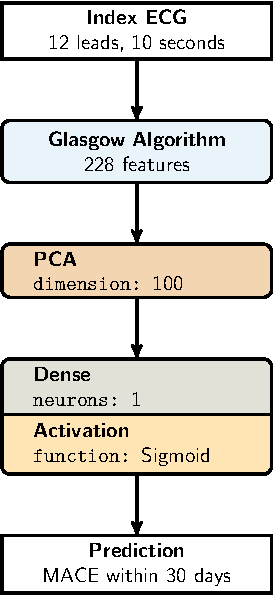
\includegraphics[scale=\modelscale,keepaspectratio]{figures/model-lr1.pdf}
\caption{Parameters and structure of the logistic regression model using only the index ECG as input.}
\end{figure}

\begin{figure}[H]
\centering
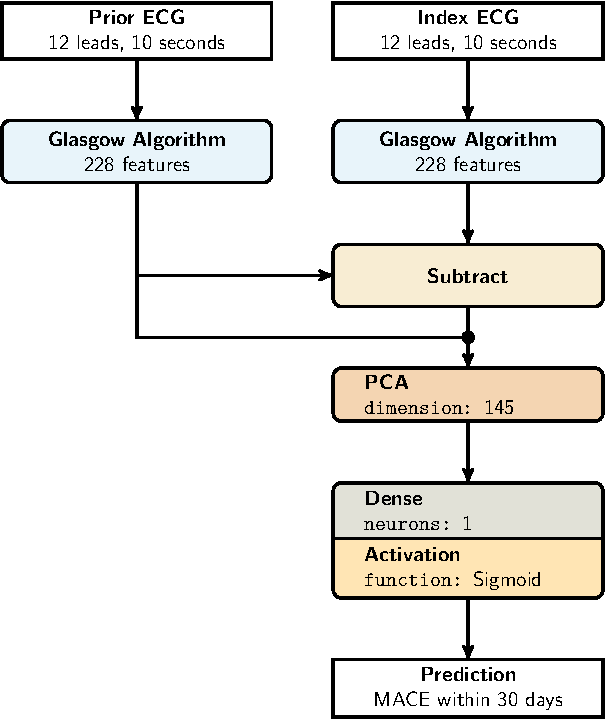
\includegraphics[scale=\modelscale,keepaspectratio,trim=0 0 -16em 0]{figures/model-lr2.pdf}
\caption{Parameters and structure of the logistic regression model using both the index and prior ECGs as input. Subtraction is vector-valued. The circle denotes concatenation.}
\end{figure}

\begin{figure}[H]
\centering
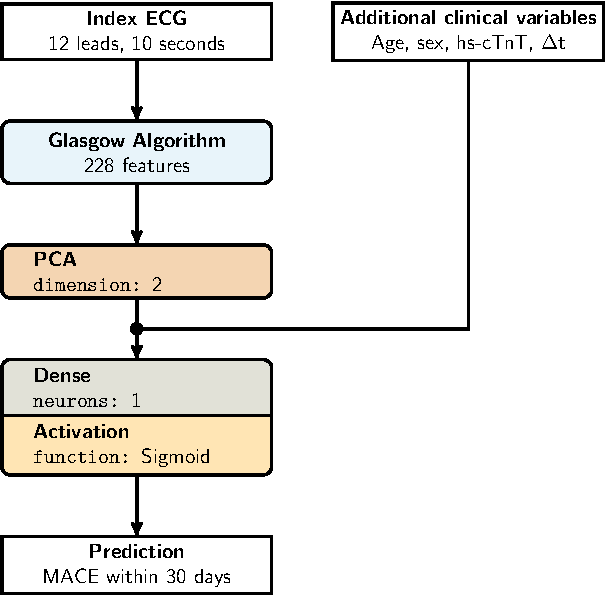
\includegraphics[scale=\modelscale,keepaspectratio,trim=-16em 0 0 0]{figures/model-lr3.pdf}
\caption{Parameters and structure of the logistic regression model using index ECG and additional clinical variables as input. $\Delta t$ is the time between the two ECGs. The circle denotes concatenation.}
\end{figure}

\begin{figure}[H]
\centering
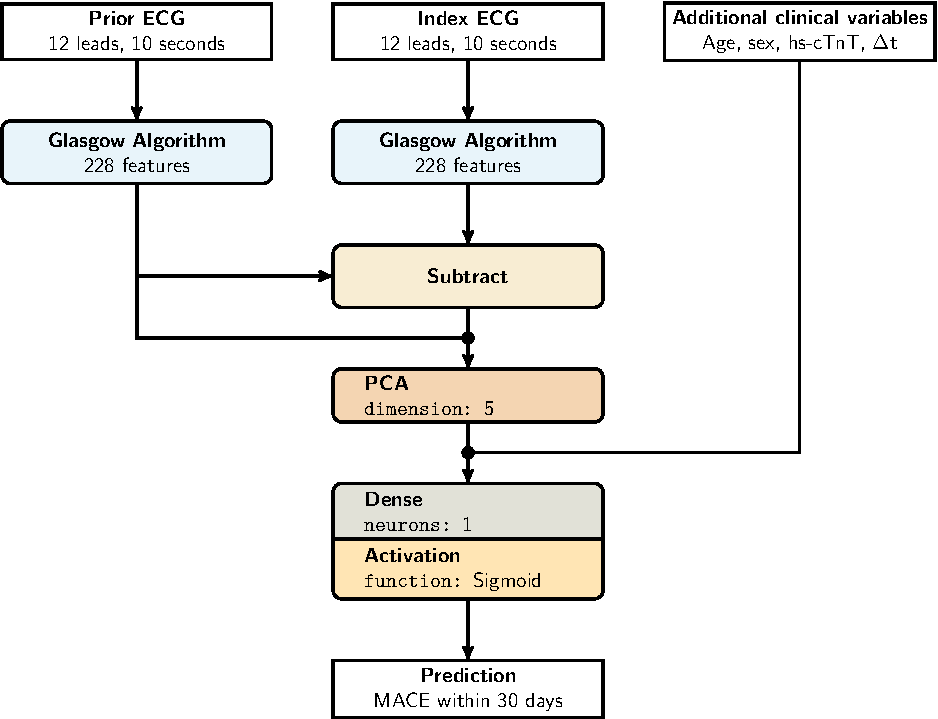
\includegraphics[scale=\modelscale,keepaspectratio]{figures/model-lr4.pdf}
\caption{Parameters and structure of the logistic regression model using both index and prior ECGs together with additional clinical variables as input. $\Delta t$ is the time between the two ECGs. Subtraction is vector-valued. The circle denotes concatenation. }
\end{figure}

\subsection{Multilayer perceptron models}
\begin{figure}[H]
\centering
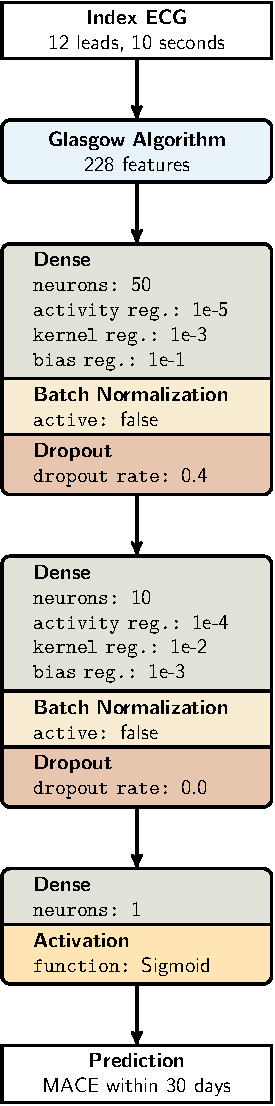
\includegraphics[scale=\modelscale,keepaspectratio]{figures/model-mlp1.pdf}
\caption{Parameters and structure of the multilayer perceptron model using only the index ECG as input. The learning rate was 0.0001.}
\end{figure}

\begin{figure}[H]
\centering
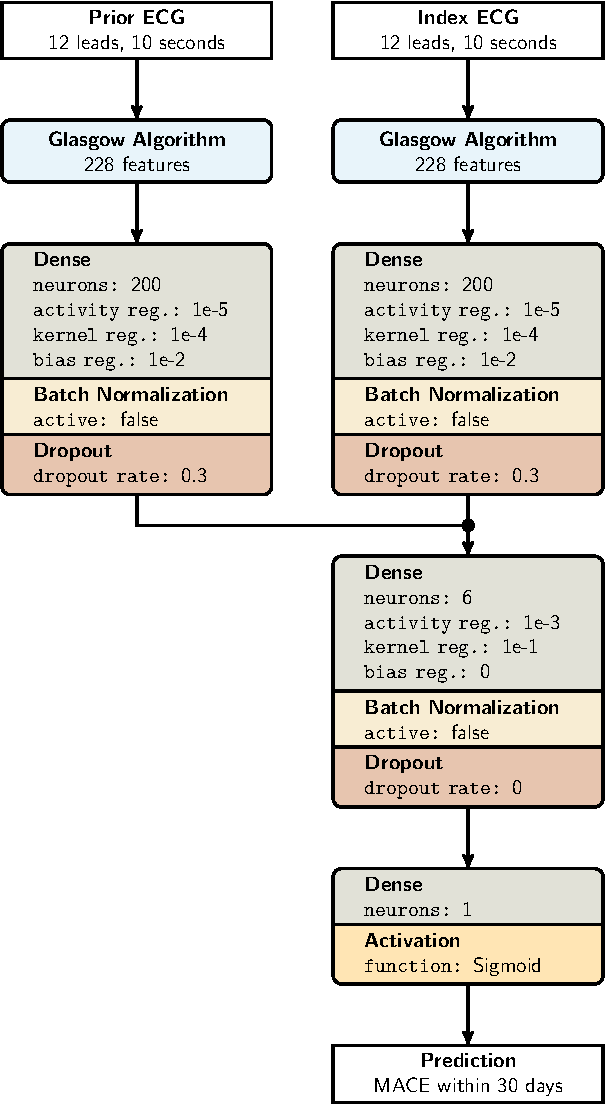
\includegraphics[scale=\modelscale,keepaspectratio,trim=0 0 -16em 0]{figures/model-mlp2.pdf}
\caption{Parameters and structure of the multilayer perceptron model using both the index and prior ECGs as input. The circle denotes concatenation. The learning rate was 0.0001.}
\end{figure}

\begin{figure}[H]
\centering
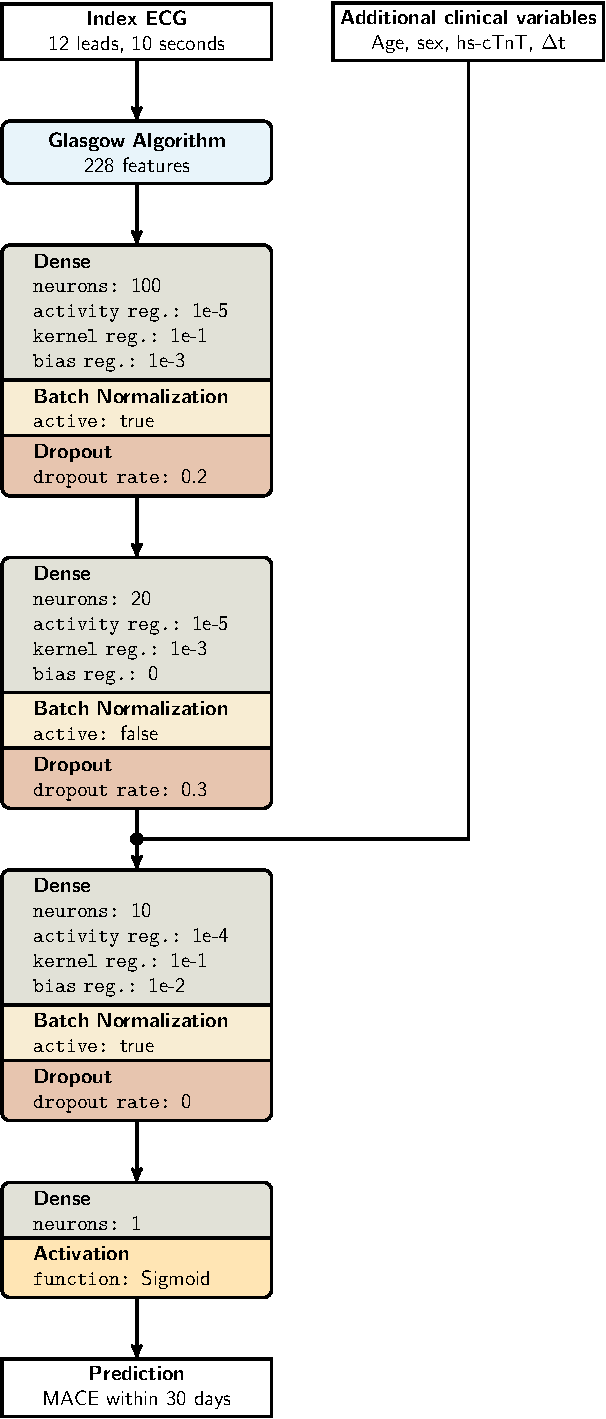
\includegraphics[scale=\modelscale,keepaspectratio,trim=-16em 0 0 0]{figures/model-mlp3.pdf}
\caption{Parameters and structure of the multilayer perceptron model using index ECG and additional clinical variables as input. $\Delta t$ is the time between the two ECGs. The circle denotes concatenation. The learning rate was 0.0003.}
\end{figure}

\begin{figure}[H]
\centering
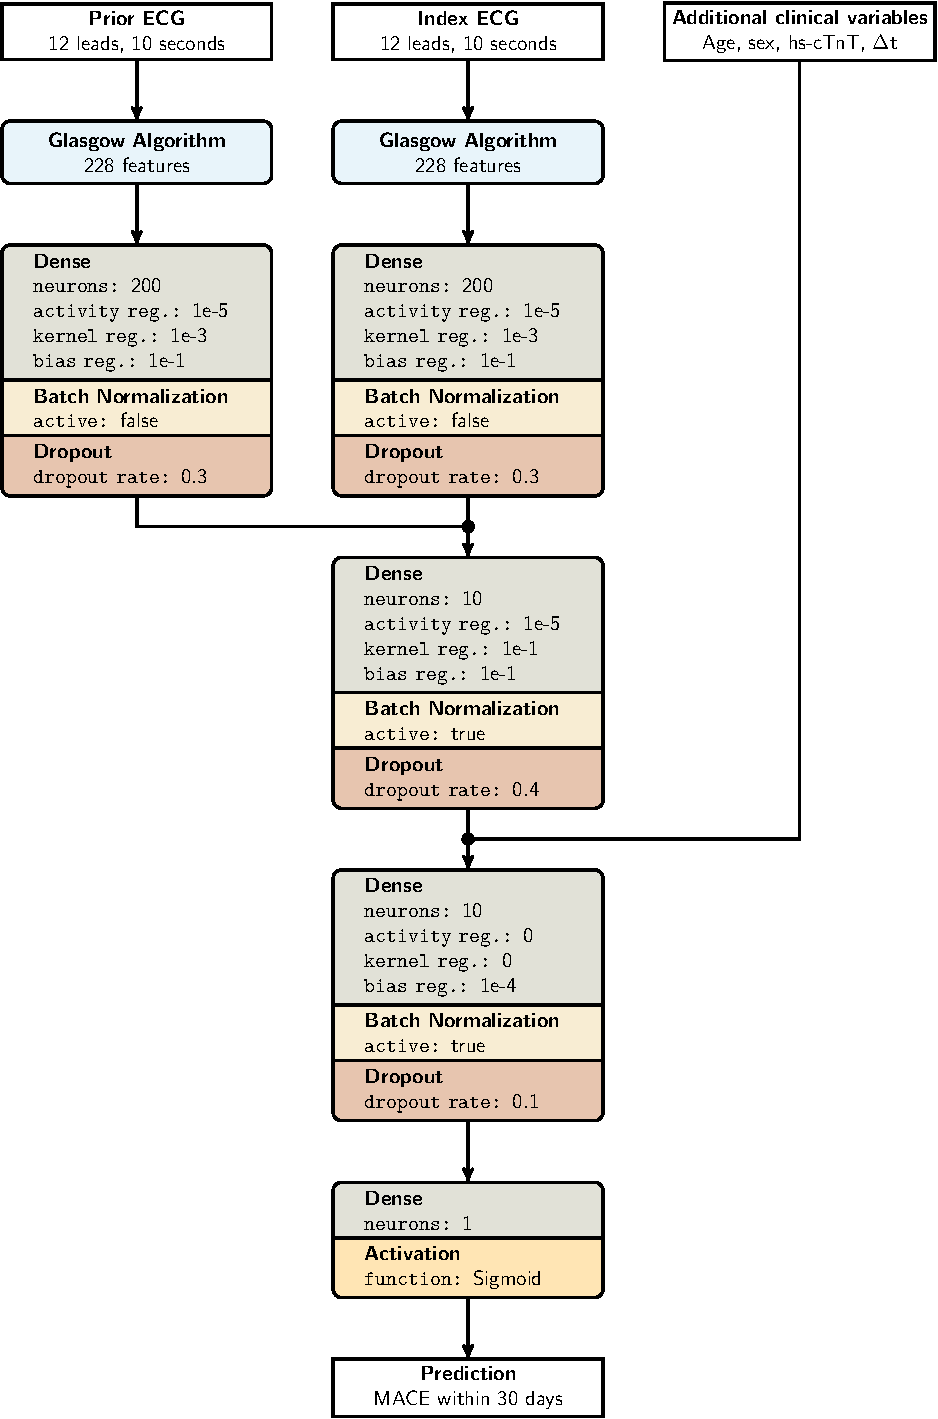
\includegraphics[scale=\modelscale,keepaspectratio]{figures/model-mlp4.pdf}
\caption{Parameters and structure of the multilayer perceptron model using both index and prior ECGs together with additional clinical variables as input. $\Delta t$ is the time between the two ECGs. The circle denotes concatenation. The learning rate was 0.001.}
\end{figure}

\subsection{Convolutional neural network models}
\begin{figure}[H]
\centering
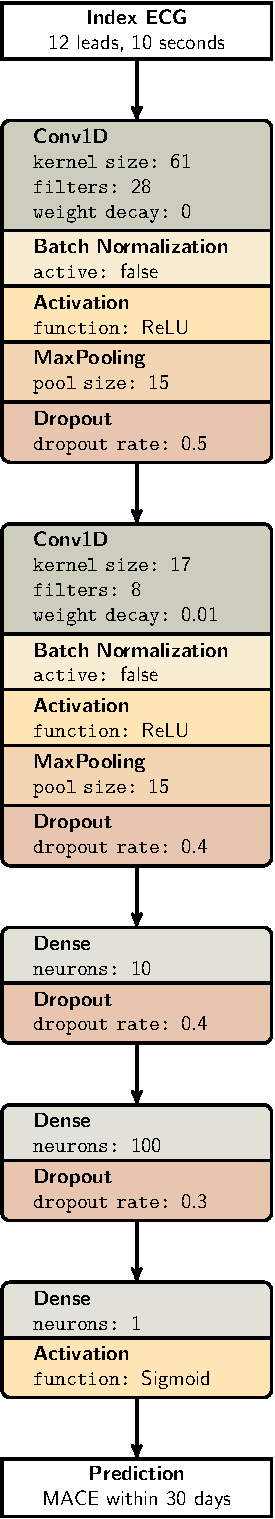
\includegraphics[scale=\modelscale,keepaspectratio]{figures/model-cnn1.pdf}
\caption{Parameters and structure of the convolutional neural network model using only the index ECG as input. The learning rate was 0.0001.}
\end{figure}

\begin{figure}[H]
\centering
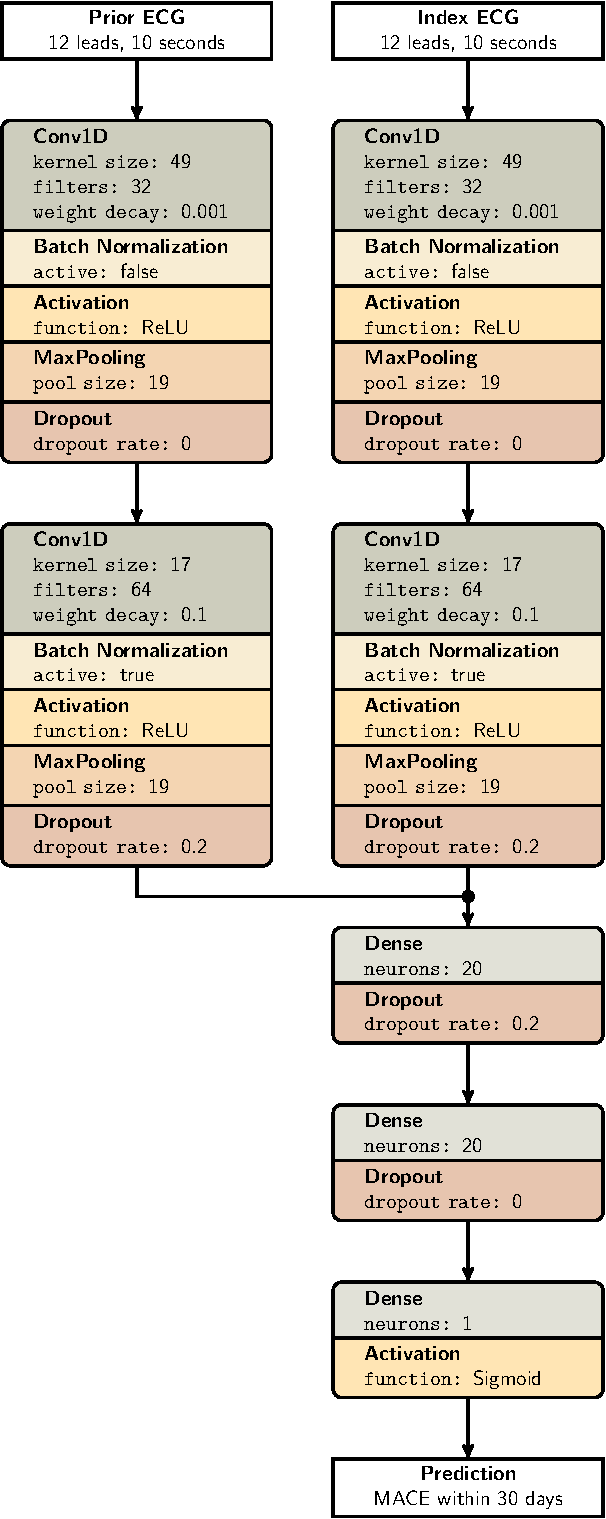
\includegraphics[scale=\modelscale,keepaspectratio,trim=0 0 -16em 0]{figures/model-cnn2.pdf}
\caption{Parameters and structure of the convolutional neural network model using both the index and prior ECGs as input. The circle denotes concatenation. The learning rate was 0.00001.}
\end{figure}

\begin{figure}[H]
\centering
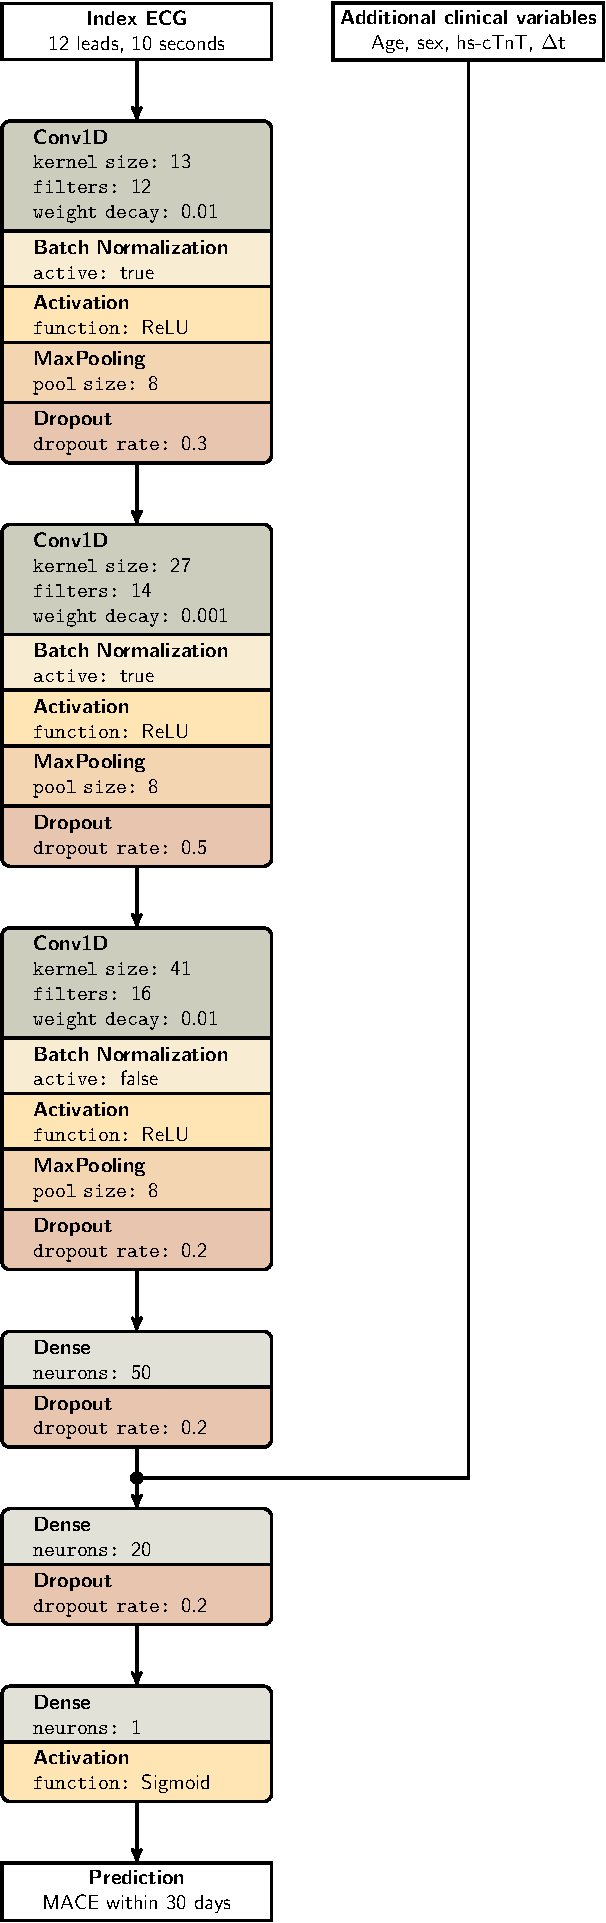
\includegraphics[scale=\modelscale,keepaspectratio,trim=-16em 0 0 0]{figures/model-cnn3.pdf}
\caption{Parameters and structure of the convolutional neural network model using index ECG and additional clinical variables as input. $\Delta t$ is the time between the two ECGs. The circle denotes concatenation. The learning rate was 0.001.}
\end{figure}

\begin{figure}[H]
\centering
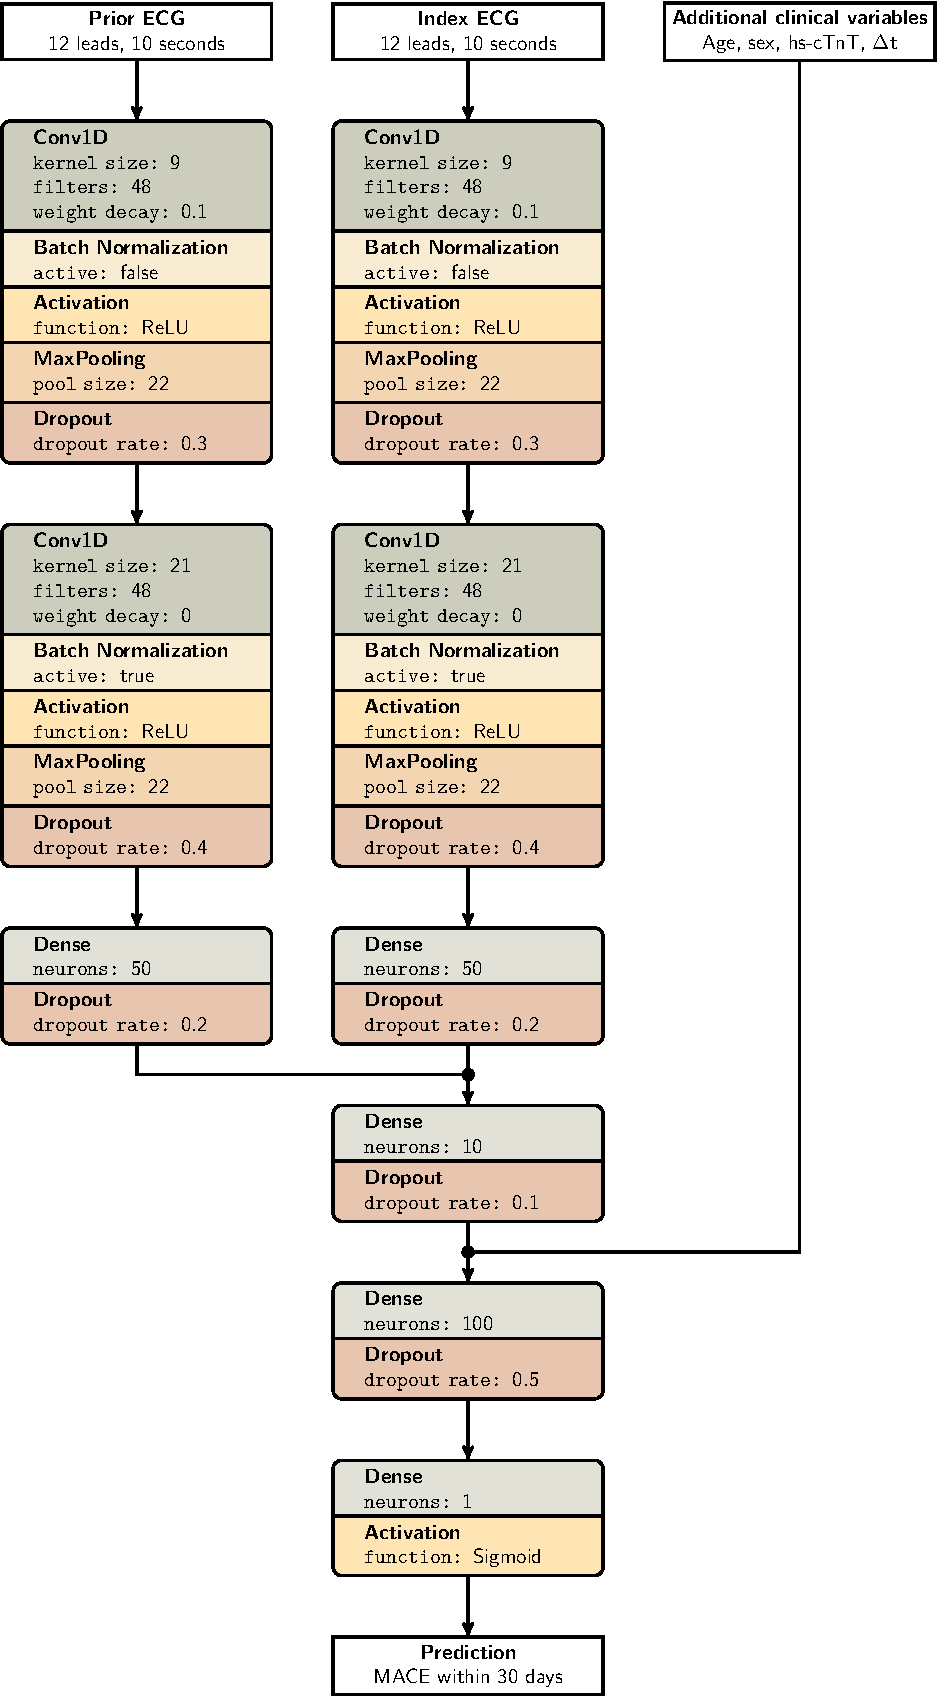
\includegraphics[scale=\modelscale,keepaspectratio]{figures/model-cnn4.pdf}
\caption{Parameters and structure of the convolutional neural network model using both index and prior ECGs together with additional clinical variables as input. $\Delta t$ is the time between the two ECGs. The circle denotes concatenation. The learning rate was 0.001.}
\end{figure}

\subsection{Residual neural network models}
\begin{figure}[H]
\centering
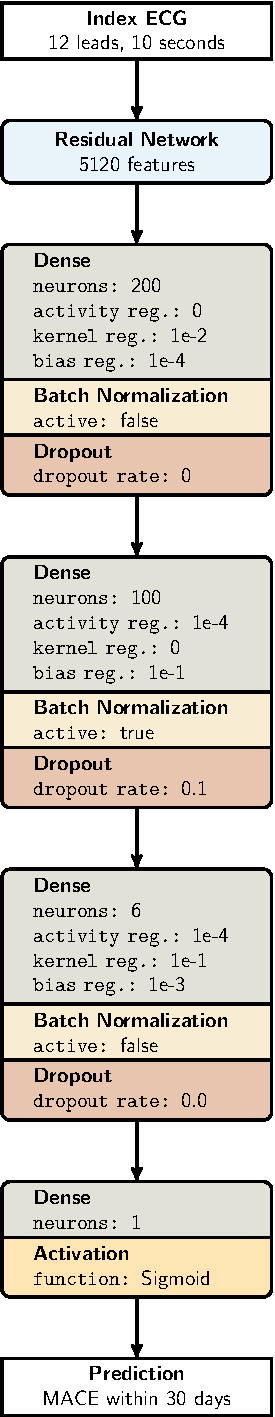
\includegraphics[scale=\modelscale,keepaspectratio]{figures/model-rn1.pdf}
\caption{Parameters and structure of the residual network model using only the index ECG as input. The learning rate was 0.0003 for all 50 epochs.}
\end{figure}

\begin{figure}[H]
\centering
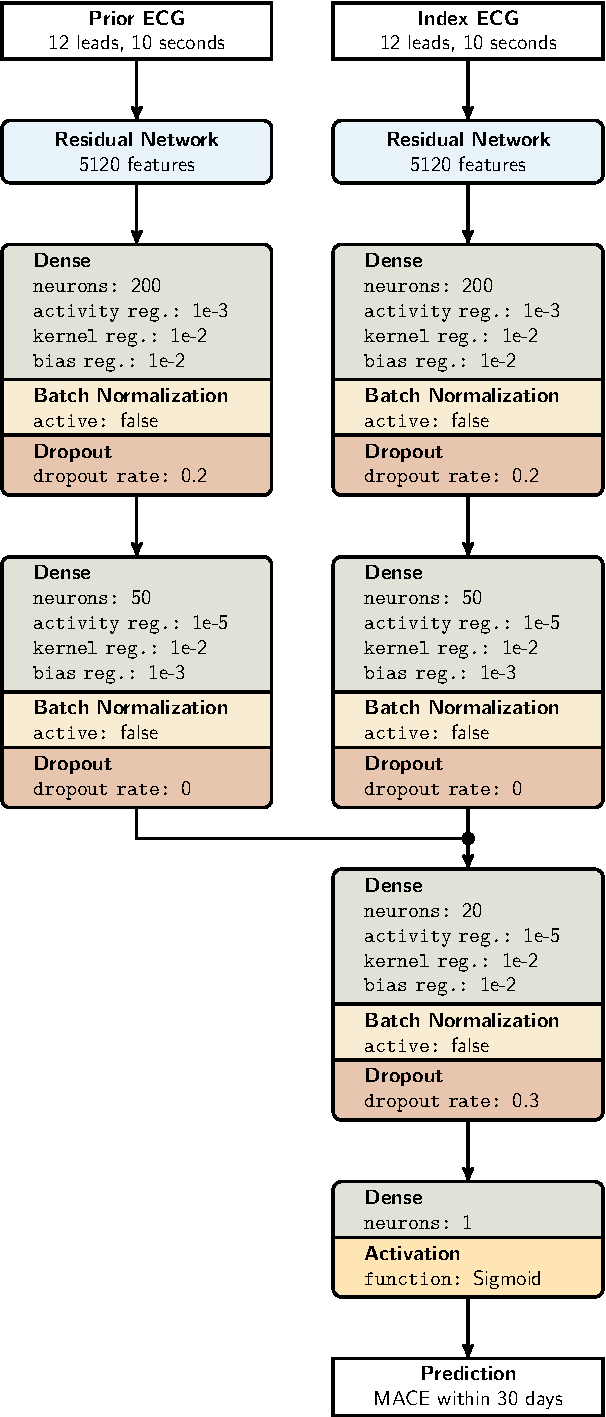
\includegraphics[scale=\modelscale,keepaspectratio,trim=0 0 -16em 0]{figures/model-rn2.pdf}
\caption{Parameters and structure of the residual network model using both the index and prior ECGs as input. The circle denotes concatenation. The learning rate was 0.001 for the first 18 epochs, and 0.00001 for the final 32 epochs.}
\end{figure}

\begin{figure}[H]
\centering
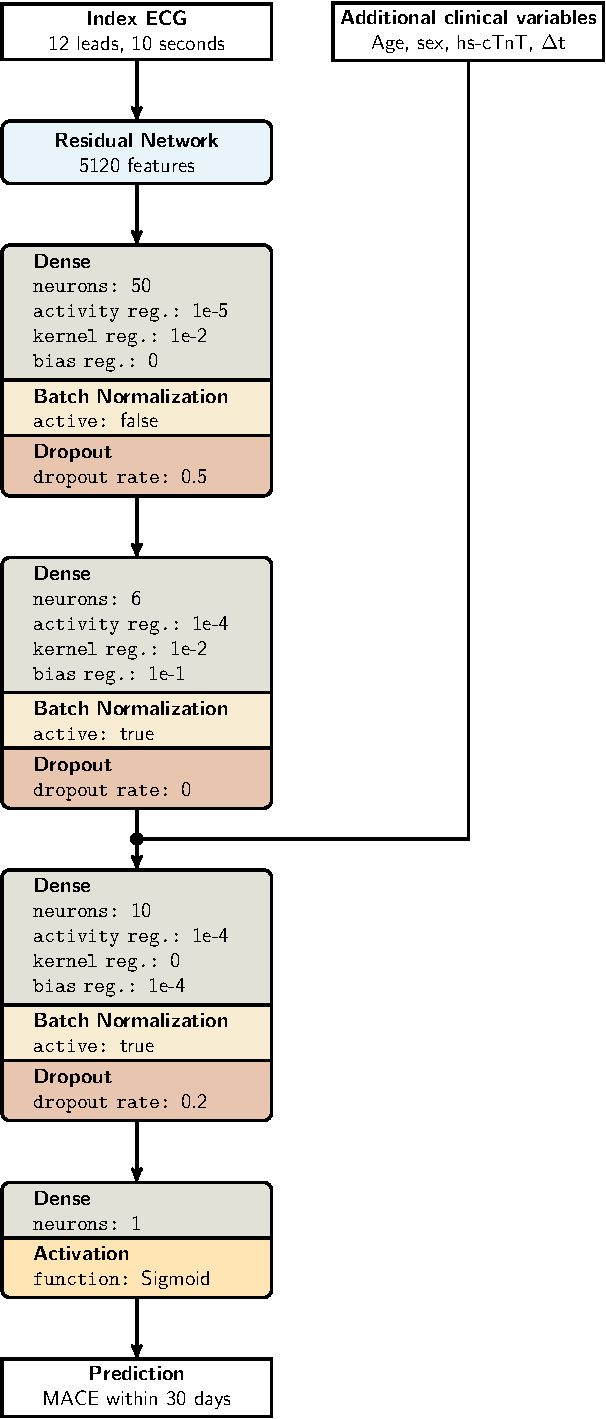
\includegraphics[scale=\modelscale,keepaspectratio,trim=-16em 0 0 0]{figures/model-rn3.pdf}
\caption{Parameters and structure of the residual network model using index ECG and additional clinical variables as input. $\Delta t$ is the time between the two ECGs. The circle denotes concatenation. The learning rate was 0.0003 for the first 24 epochs, and 0.00003 for the final 26 epochs.}
\end{figure}

\begin{figure}[H]
\centering
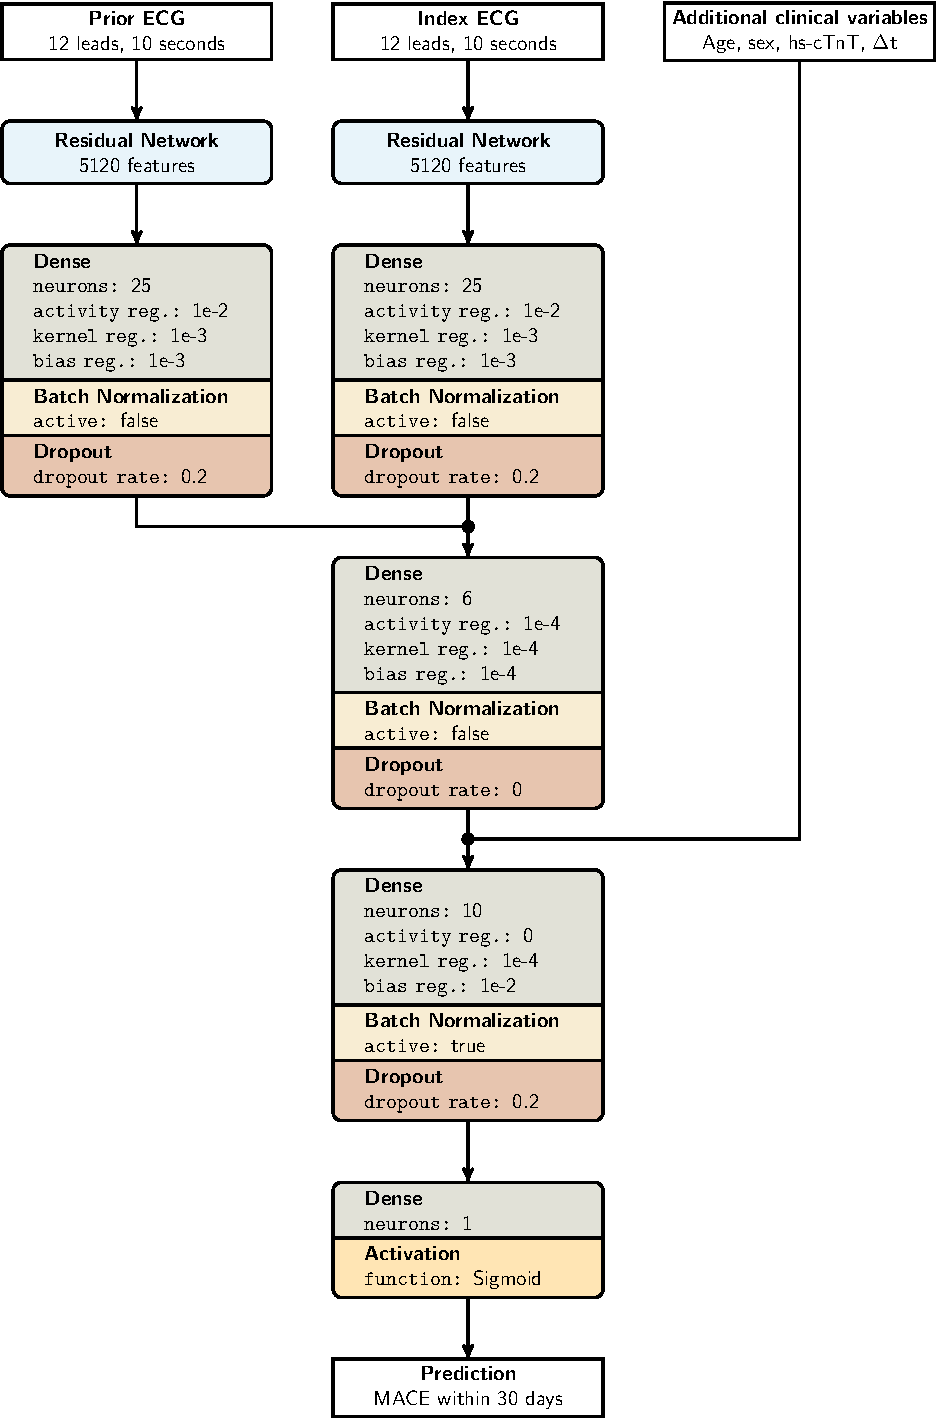
\includegraphics[scale=\modelscale,keepaspectratio]{figures/model-rn4.pdf}
\caption{Parameters for and structure of the residual network model using both index and prior ECGs together with additional clinical variables as input. $\Delta t$ is the time between the two ECGs. The circle denotes concatenation. The learning rate was 0.003 for the first 33 epochs, and 0.00001 for the final 17 epochs.}
\end{figure}

\bibliography{supplement}

\end{document}
